The main study was designed to validate the results of the pilot study over different locations at different times. 
We choose five different locations across central London, to install the sensors and collect data for a long period of time. 
We also carry out manual counting on these locations along with this across different time of the day. 
We then apply the filtering based on signal strength and sequence numbers and compare with manual counts and evaluate the effectiveness of the process with the mean error per minute on these locations. 
Finally we calculate the ajustment factor for the first interval of manual counts and check if that works on the consecutive intervals. 

The locations where the data were collected are shown in the table. The location are chosen for their variety of configuration and sources of noise. Location 1 is the `cleanest' of while location 2 is the one with the most complexity. The configuration, installation and data collection schedule is shown in the figure. 

\begin{figure}
	\begin{center}
		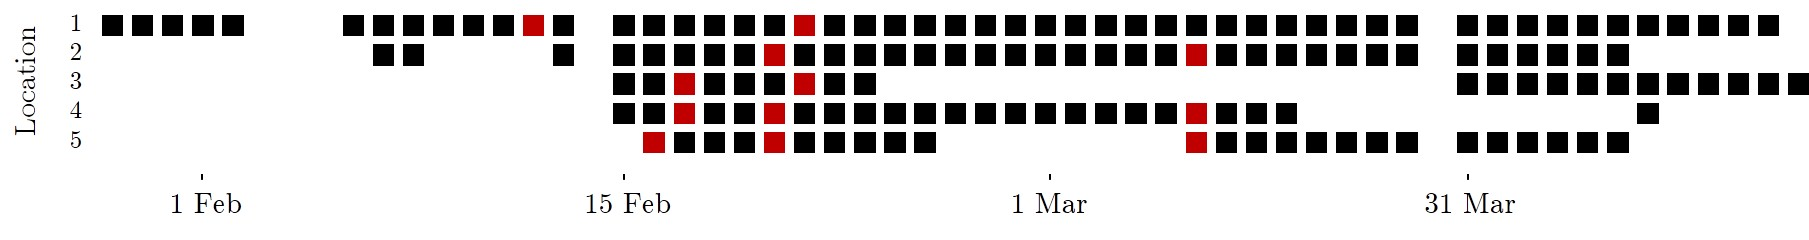
\includegraphics [width=\linewidth] {images/main_schedule.jpeg}
		\caption{Clustering probe requests based on increasing sequence numbers present in them. The dots are individual probe requests and the red lines connect probe requests within the same cluster which are generated by the same mobile device.}
		\label{pilot_clustering}
	\end{center}
\end{figure}

\begin{table}
	\tbl{Locations where sensors were installed}
	{\begin{tabular}{clll} 
		\toprule
		 ID & Location & Type & Installation notes\\
		 \midrule
		 1 & Camden High Street & Phone Shop & Bus stop in front\\
		 2 & Central St.Giles Piazza & Restaurant & Seating area on both sides\\
		 3 & Holborn Underground Station & Information Kiosk & Overlooks station entrance\\
		 4 & Brunswick Center & Fast Food Restaurant & Has seating area on one side\\
		 5 & The Strand & Regular Shop & Has phone shop next door \\
		 \bottomrule
	\end{tabular}}
	% \tabnote{\textsuperscript{a}This footnote shows how to include footnotes to a table if required.}
	\label{locations-table}
\end{table}

\begin{figure}
	\centering
	\subfigure[Distribution of signal strengths showing the filtering of background noise]{
		\resizebox*{0.46\linewidth}{!}{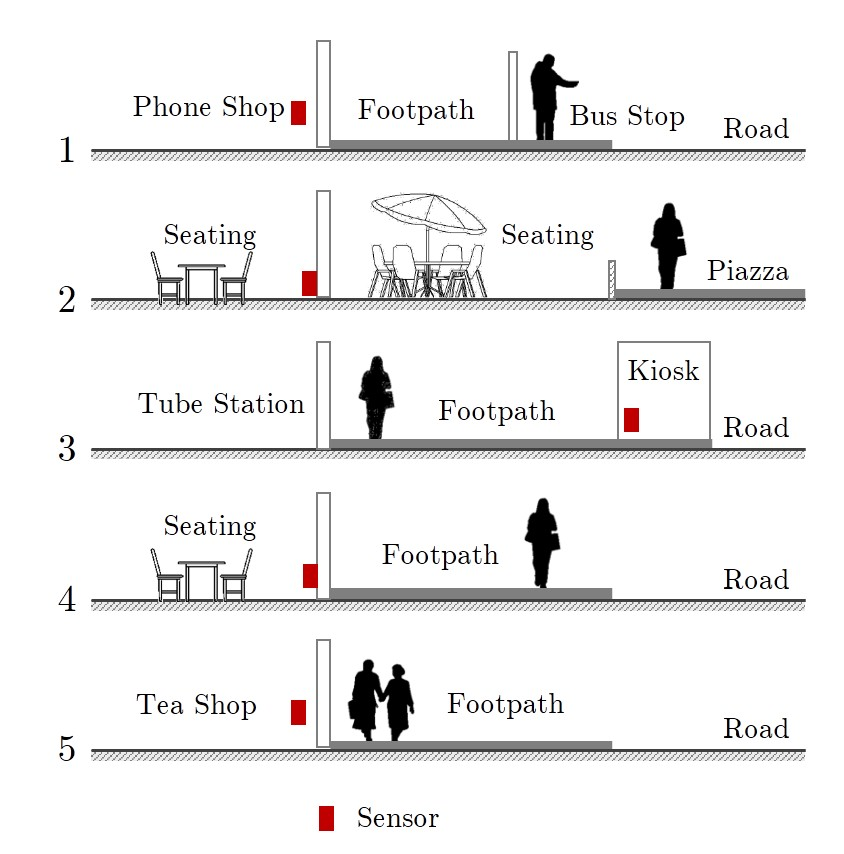
\includegraphics[trim=20 6 20 6,clip]{images/main_configs.jpeg}}}\hspace{20pt}
	\subfigure[Clustering probe requests as nodes in a graph using increasing sequence numbers]{
		\resizebox*{0.46\linewidth}{!}{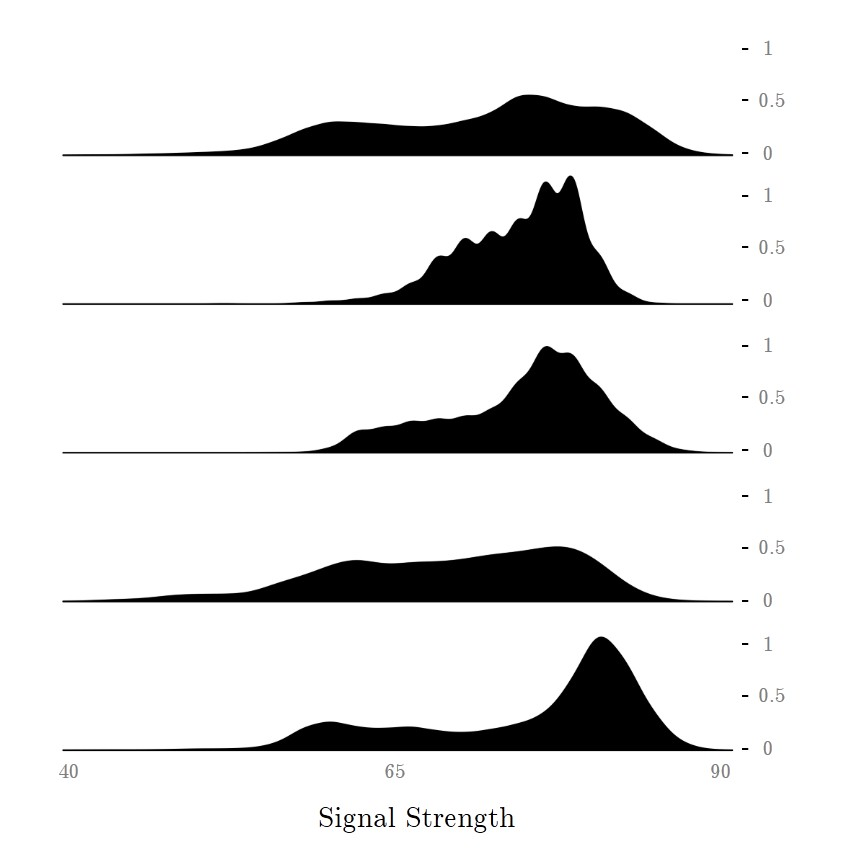
\includegraphics[trim=20 6 25 6,clip]{images/main_signals.jpeg}}}
	\caption{Schematic diagrams explaining the methods for filtering by signal strength and clustering using sequence numbers} \label{methodology_schematic}
\end{figure}

The comparision between global and local.
comparision between different types of vendors.
Specifics on top 5 manufacturers.

We do a daily analysis of distribution of signal strengths.
The thresholds are shown in the table.
The average is xxxx and standard deviation is xxx.
we notice that the variation is lot. There is a definite
change with the micro site locations.

We see how the signal strength filtering affects the counts.
compared to manual counts we look at the average mean errors (daily)
per 5 minutes. The counts go as follows.
Shown as a red line in the Figure.

We can conclude that even though it has variations, this is
a good method to reduce the overall level of error.

This is also done for different locations hourly for all the data we had.
we compare it to the manual counts and see that the average mean error
has been reduced/increased. The finger print works well for all the locations.
It also works over a period of time and gives us a comparable and close 
footfall count to the manual count. The thresholds found in the pilot study
works as well.

Finally we normalise the sensor counts to match the manual count using
a fraction/ adjustment factor calculated from the know manual counts.
we have three sets of counts. We check if the adjustment factor holds the
same in all three counts across locations. It does with a variations from
xxx to xxx. The results are shown in the table. 

we see that the signal strength filtering works and reduces error by
xxxxx. there is variation by locations.
we see that sequence number algorithm works as well. The threshold stays
constant well and works well across locations. The calibration also works
and ajustment factor stays consistent short term. This needs more work 
long term.
